\documentclass[review]{elsarticle}

\usepackage{lineno,hyperref,ulem,todonotes}

\modulolinenumbers[5]
%\usepackage{natbib}
%\journal{Journal of \LaTeX\ Templates}

%%%%%%%%%%%%%%%%%%%%%%%
%% Elsevier bibliography styles
%%%%%%%%%%%%%%%%%%%%%%%
%% To change the style, put a % in front of the second line of the current style and
%% remove the % from the second line of the style you would like to use.
%%%%%%%%%%%%%%%%%%%%%%%

%% Numbered
\bibliographystyle{model1-num-names}

%% Numbered without titles
%\bibliographystyle{model1a-num-names}

%% Harvard
%\bibliographystyle{model2-names.bst}\biboptions{authoryear}

%% Vancouver numbered
%\usepackage{numcompress}\bibliographystyle{model3-num-names}

%% Vancouver name/year
%\usepackage{numcompress}\bibliographystyle{model4-names}\biboptions{authoryear}

%% APA style
%\bibliographystyle{model5-names}\biboptions{authoryear}

%% AMA style
%\usepackage{numcompress}\bibliographystyle{model6-num-names}

%% `Elsevier LaTeX' style
%\bibliographystyle{elsarticle-num}
%%%%%%%%%%%%%%%%%%%%%%%

\begin{document}

\begin{frontmatter}

\title{A mixed-dimensional model for the simulation of soil thermal hydrology in polygonal tundra}
%\tnotetext[mytitlenote]{Fully documented templates are available in the elsarticle package on \href{http://www.ctan.org/tex-archive/macros/latex/contrib/elsarticle}{CTAN}.}

%% Group authors per affiliation:
%\author{Elsevier\fnref{myfootnote}}
%\address{Radarweg 29, Amsterdam}
%\fntext[myfootnote]{Since 1880.}

%% or include affiliations in footnotes:
%\author[mymainaddress,mysecondaryaddress]{Elsevier Inc}
%\ead[url]{www.elsevier.com}

%\author[mysecondaryaddress]{Global Customer Service\corref{mycorrespondingauthor}}
%\cortext[mycorrespondingauthor]{Corresponding author}
%\ead{support@elsevier.com}

%\address[mymainaddress]{1600 John F Kennedy Boulevard, Philadelphia}
%\address[mysecondaryaddress]{360 Park Avenue South, New York}

\begin{abstract}
Permafrost soils harbor massive amount of frozen organic carbon and are warming at a rate significantly larger than the rest of the planet. Modeling and simulation techniques are essential tools for studying the complex hydrological environment of the Arctic regions. These tools help to determine the responses of the Arctic ecosystems to changing climate. \\
We present a novel mixed-dimensional model, motivated by fine-scale simulations, to simulate soil thermal hydrology in degrading permafrost regions and make these process-rich simulations tractable at watershed scales. The approach indirectly couples one-dimensional subsurface columns with a two-dimensional surface system, and has two fundamental steps. Step 1 solves overland thermal hydrology system with no sources, mainly act as a spatial distributor of the mass and energy, and updates the subsurface system before it advances in time. Step 2 implicitly solves the subsurface system with surface ponding but no surface lateral flow, and use the output of that half-step to update the pressure and temperature of Step 1 for the next iteration. \\
This is a first attempt to couple state-of-the-art representation of freezing soil physics with overland flow and surface energy balance at scales of 100s of meters. 
We demonstrate the accuracy and efficiency of our scheme. Our scheme is highly scalable, supports subcycling of different processes, and compares well with fully 3D representation, but is computationally less expensive. Further, it allows for efficient tracking of thaw-induced subsidence and avoids any mesh tangling that can result from representing dynamic topography in a 3D simulation. Although we focus on permafrost thermal hydrology, the model structure is applicable to many integrated surface and subsurface thermal hydrology problems at field-scale.
% to simulate the thermal hydrology of thawing polygonal tundra near Barrow, Alaska in warming climate.
\end{abstract}

\begin{keyword}
Mixed-dimensional model\sep Permafrost dynamics  \sep Process-rich simulations \sep Arctic 
%\MSC[2010] 00-01\sep  99-00
\end{keyword}
\end{frontmatter}

\linenumbers

\section{Introduction}

Permafrost soils, perennially frozen ground, are large carbon pools and reservoirs. Approximately 23\% of the land surface in the Northern Hemisphere is covered by continuous permafrost (91-100\% frozen area), and another 17\% is occupied by discontinuous permafrost (50-90\% frozen area)~\cite{brown1997circum,jorgenson2001permafrost}. A massive amount of organic carbon (approximately 1672 Pg) is stored in the Northern Hemisphere and these high-latitude regions are warming at a rate considerably faster than most of the world~\cite{tarnocai2009soil, turner2007arctic, hansen1999giss, assessment2004impacts}. In a warming climate, permafrost regions are under potential risk of carbon release to the atmosphere and can transform from a carbon sink to a carbon source -- that could increase the concentration of carbon in the atmosphere, which in turn would lead to further increase in the temperature~\cite{billings1982arctic}. Thawing of permafrost and thereby it's considerable degradation can cause significant changes in the surface and subsurface thermal hydrology and eventually can substantially alter the Arctic tundra ecosystems~\cite{osterkamp1983response, walvoord2007increased, lyon2009estimation, pachauri2014climate,koven2013analysis}. Therefore, due to increasing computing power, modeling and simulation techniques turned to be useful and reliable tools that should be used to gain more insight into the role of permafrost degradation in temperature-sensitive Arctic ecosystems and to accurately project the consequent changes at larger spatial and temporal scales.

There has been a great interest in studying permafrost dynamics in warming climate through modeling and simulation techniques. Though such techniques help to better understand the role of soil warming, responses of tundra ecosystems to warming trends, and to further expose the corresponding consequences on the degradation of permafrost and the associated changes in the surface and subsurface thermal hydrology. However, simulating permafrost dynamics in a complex and coupled surface/subsurface thermal hydrological environment is a hard and challenging task, particularly, at larger spatiotemporal scales; see~\cite{painter2013modeling}. Pertinent to literature, early research efforts mostly focused on one-dimensional simulations of subsurface thermal hydrology, for example,~\cite{harlan1973analysis, guymon1974coupled, taylor1978model}. In previous decade, some studies were directed to demonstrate coarse-scale surface modeling techniques~\cite{takata2003development, nicolsky2007improved, mckenzie2007groundwater}. More recently a few studies demonstrated two- and three-dimensional simulations of permafrost dynamics with simplified (or subsurface only) models; see~\cite{bense2009evolution, lawrence2012simulation, koven2013analysis, karra2014three}. A comprehensive review of the published modeling efforts of the surface and subsurface can be found in~\cite{kurylyk2014climate}. It is worth pointing out that mathematical models with limited complexity, relatively coarse resolutions etc. provide some insight into permafrost dynamics but do not accurately represent Arctic ecosystems. The process-rich based simulations are essential to accurately capture the potential impacts of permafrost thawing on the surface and subsurface thermal hydrology and the consequent changes.

In light of the above discussion, we need sophisticated hydrological computer codes to simulate fully integrated surface and subsurface system and process-rich complex models over long spatiotemporal domains. However, as said earlier, simulating soil thermal hydrology in degrading permafrost regions is challenging due to strong coupling among thermal and hydrologic processes on the surface and in the subsurface, thaw-induced subsidence, complex microtopographic features (i.e., topography at the scale of polygons) etc. One of the challenges is a small time-step issue during phase transition. Frozen subsurface is less permeable and blocks infiltration, as ice begins to melt (phase change occurs), the soil hydraulic conductivity increases, consequently, the time-step of numerical methods decreases \cite{dall2011robust}. To ensure a long-term projection, a small time-step is not practical, because a huge amount of computational time is spent in recovering the time-step, which may not recover in a reasonable amount of time. The other major challenge is tracking thaw-induced subsidence. Most of the existing hydrological simulators are mainly designed to conduct three-dimensional simulations, however, deformations in a three-dimensional simulation are not easy to track due to mesh tangling and could cost huge computational burden, further, a poor mesh quality may question accuracy of the results. In addition, lack of flexibility and extensibility of the simulators also limit and discourage future extensions.

To address the aforementioned challenges, we present a novel modeling strategy for process-rich simulations of integrated surface and subsurface thermal hydrology in lowland tundra systems with low topographic gradients. We focus on polygonal tundra, large and carbon-rich regions of northern Siberia, Alaska, and Canada where soil cracking has led to the formation of subsurface ice wedges that honeycomb the subsurface and tesselate the land surface into polygonal patterns. Rather than solve a fully three-dimensional subsurface system tightly coupled to surface processes as in \cite{spainter2106integrated}, we take advantage of physical insights gained from fine-scale simulations and approximate the integrated surface/subsurface dynamics with mutually independent 1-D columns, each associated with an ice wedge polygon. The columns are then sequentially coupled to a surface thermal flow system. Mixed dimensional model structures have been used previously in simulations of variably saturated flow at watershed scales, in particular to couple multiple 1-D unsaturated (vadose) zone representations to a two- or three-dimensional saturated zone; for example see~\cite{pikul1974numerical,zhu2011method}. Here we apply the mixed-dimensional model structure to an integrated surface/subsurface flow system including surface and subsurface thermal processes and evaluate the accuracy and computational advantages of the approximation. 

This mixed-dimensional modeling approach is motivated by some fine-scale simulations at the ice-wedge polygon scale that showed that differences in the thermal conditions among centers, rims and troughs of ice-wedge polygons are largely equilibrated by lateral heat transport during summer such that the system behaves similarly to a one-dimensional system at seasonal time scales. 

We have implemented our mixed-dimensional modeling strategy in an open-source state-of-the-art software known as Advanced Terrestrial Simulator (ATS) 
~\cite{ecoon2016managing, spainter2016integrated}. Particularly related to this work, ATS solves strongly coupled surface energy balance, and surface and subsurface thermal hydrology in a highly parallel 3D environment. We present details about the ATS in later sections, but it is mainly a collection of PKs and MPCs. A PK (Process-Kernel) refers to a mathematical model, and MPC stands for Multiprocess Coordinator that couples different PKs, that is, it facilitates communication among individual PKs.

The paper is organized as follows: Section~\ref{motivation} presents some fine-scale simulations' results and analysis that motivated the approach. Section~\ref{arcos-framework} highlights the Arctic Terrestrial Simulator (ATS) and the Arcos framework for the implementation of the model. In Section~\ref{mixed-dim-model} we introduce our mixed-dimensional modeling approach, loosely coupled scheme and the ATS refactoring strategy. To illustrate the performance and efficiency of our modeling strategy, in Section~\ref{numerical-tests} we compare our numerical results with the three-dimensional simulations based on strong coupling, and present speedup and scalability of the new technique. Concluding remarks and future research are offered in Section~\ref{conclusion}, followed by references.

%\section{Motivation and Modeling Approach}\label{motivation}

\section{Motivation: Fine-scale Simulation Study}\label{motivation}

Our mixed-dimensional approach is motivated by the results of fine-scale two-dimensional simulations on vertical cross-sections across ice-wedge polygons at the Barrow Environmental Observatory. The simulations coupled a surface energy balance model with and without snow, snow distribution models, models for thermal overland flow including phase change, and a recently developed three-phase subsurface thermal hydrology model. The soil properties were calibrated against borehole temperature data in a previous study \cite{atchley2015}. The simulations were forced with meteorological data for the site. Those simulations used an unstructured mesh that conforms to surface topography derived from lidar measurements. Horizontal mesh resolution is approximately 0.25 m. Vertical resolution is 0.02 cm at the surface and gradually increases with depth. Details on boundary conditions and the spinup process can be found in \cite{spainter2016integrated}. 

Snapshots of ice and liquid saturation indices in cross-section across two ice-wedge polygons are shown in Fig.~\ref{oct15}. These snapshots are for October 15, 2013, which is during the fall freeze-up. During this period, the rims of the ice-wedge polygons are significantly colder than the centers and troughs because the thermally insulating snowpack is smaller on the rims. Previous one-dimensional simulations~\cite{atchley2016} have shown that thermal differences caused by differences in snow depth lead to differences in active layer thickness, the depth of the annual thaw. However, in the two-dimensional simulations shown here, the active layer thickness shows little variation across the polygon (Fig.~\ref{alt}). Although transient differences in subsurface temperature occur due to differences in snow depth, soil moisture content, and albedo, lateral heat transport is sufficient to equilibrate those differences by the time of maximum thaw. Thus, the active layer thickness, which is a primary control on the annual carbon decomposition rates, is not directly affected by microtopographic position within an ice-wedge polygon. This lack of sensitivity suggests a model structure where the ice-wedge polygon becomes the unit computational cell on the surface. 

\begin{figure}[!htpb]
\centering
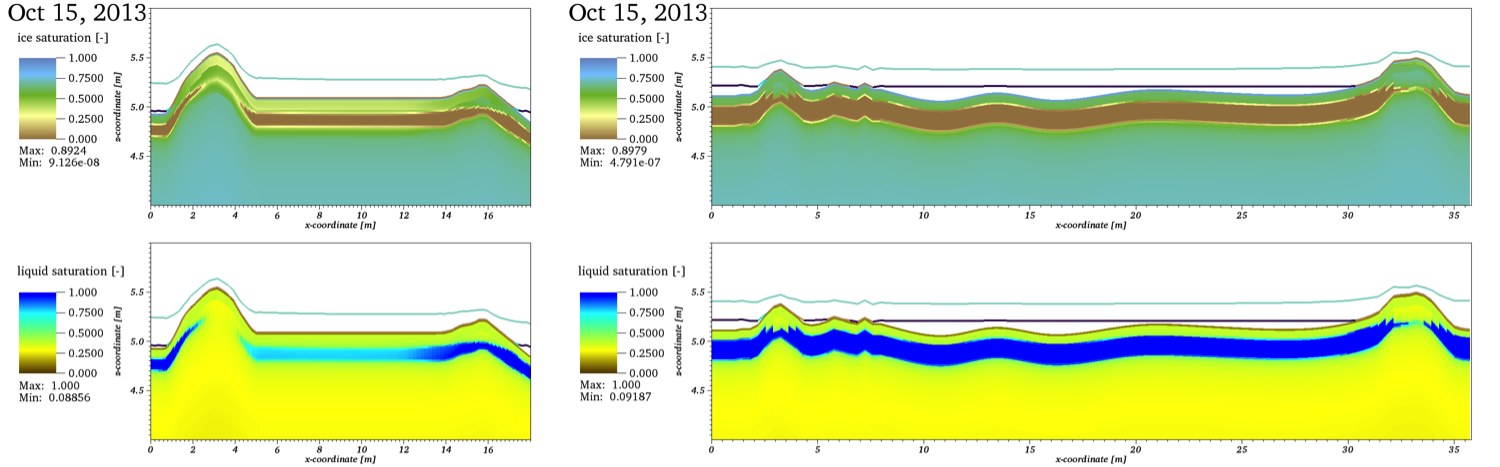
\includegraphics[width=15cm]{figures/FineScaleOct15.png}
\caption{Results from two-dimensional fine-scale modeling. Shown are snapshots of ice saturation index and liquid saturation index in cross-sections across two ice-wedge polygons.}
\label{oct15}
\end{figure}

\begin{figure}[!htpb]
\centering
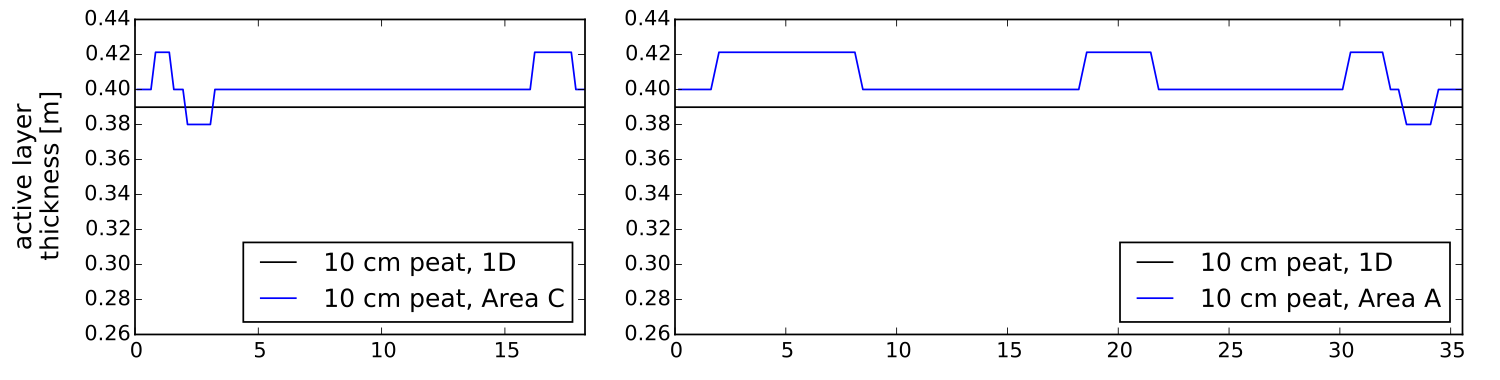
\includegraphics[width=10cm]{figures/ALT-finescale.png}
\caption{Active layer thickness from fine-scale modeling}
\label{alt}
\end{figure}

\section{Arcos Framework}\label{arcos-framework}

As stated earlier, studying permafrost dynamics at large-scale is an important challenge, and requires simulators to be capable of handling many surface and subsurface processes, and the mutual interactions among them. Most existing hydrological computer codes, in the context of implicit-based coupling among processes, and the implementation architecture, don't efficiently allow and encourage modelers to study permafrost evolution at larger spatial and temporal scales. These simulators lack the flexibility of future development for extensions, that is, incorporating more processes and/or increasing the complexity of existing models for accurate representation of reality (e.g., changes in the Arctic ecosystem and predictability of carbon emissions and its content to the atmosphere in warming climate) is not a trivial task.

The Arcos framework enhances modeling capabilities more efficiently than existing simulators, and offers flexible process-rich simulations' environment to address challenging problems such as permafrost degradation. The Arcos framework manages the process kernels (a mathematical model) in a hierarchical way (i.e., process tree form). In other words, the Arcos framework provides an architecture that manages multiphysics models and allow them to interact through a Multiprocess Coordinator (MPC). This hierarchical structure keeps the implementation of each mathematical model isolated that can be coupled with many other models through an MPC. Due to this flexibility and significant extensibility, the Arcos framework-based simulators provide ideal modeling environment, tackle the complexities efficiently, and encourage future extensions. 
In this study, we use publicly available state-of-the-art computer code the Advanced Terrestrial Simulator (ATS). The ATS is inherited from Amanzi -- Amanzi is a flow and reactive transport simulator mainly build on the Arcos framework~\cite{moulton2012high}. In subsequent sections, we describe how we refactored the ATS for our modeling technique. More details about the ATS and Amanzi are available in~\cite{ecoon2016managing, moulton2012high, spainter2016integrated}.


\section{Modeling Approach, Coupling Scheme, and ATS Refactoring Strategy}\label{mixed-dim-model}

In this section, we first describe the mixed-dimensional modeling approach then present the weakly coupled scheme followed by the refactoring strategy of the ATS.
\subsection{Mixed-Dimensional Modeling Approach}
Technically, our modeling strategy splits a 3D domain into $2N+1$ subdomains, where $N$ is the total number of surface elements. The total $2N+1$ subdomains include $N$ subdomains for 1D subsurface columns, one subdomain for the 2D overland system, and there are also $N$ 1D surface cells placed upon each 1D subsurface column for water ponding and forcing data (e.g., rain precipitation, air temperature, wind speed etc.) To avoid confusion, hereafter the 2D overland system is referred to as surface-star system, and the 1D surface cells will collectively be called surface system. The 1D columns and surface-star system is highlighted in Fig.~\ref{surf-cols}. The $2N+1$ subdomains form a complex PK tree with $2N+1$ processes as illustrated in Fig.~\ref{pk-tree}. The PK tree consists of independent, strongly and weakly coupled PKs highlighted in light blue, light cyan, and orange colors, respectively. In our approach, the interaction at the interface between the surface-star and 1D columns happens at the top level weak MPC. The strong MPC (on the left at the second level) is the surface-star system. The weak MPC at the second level iterates over all the surface and subsurface subdomains. The PK-I, I $=1,2,3, \dots, N$ denote integrated surface (a cell) and subsurface (1D column) system. The tree attached to the black octagon shape is replicated across all PK-I, I $=1,2,3, \dots, N$.

\begin{figure}[!htpb]
\centering
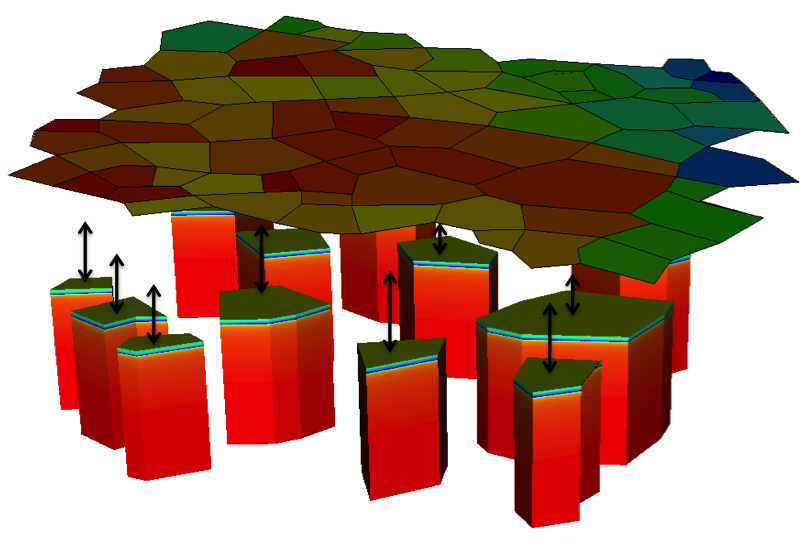
\includegraphics[height = 7.5cm, width=10cm]{figures/mixed-dim-model.png}
\caption{An illustration of the independent 1D subsurface columns coupled to the surface-star system. The surface system (1D cells lying on the top of corresponding columns) are not shown.}
\label{surf-cols}
\end{figure}


\begin{figure}[!htpb]
\centering
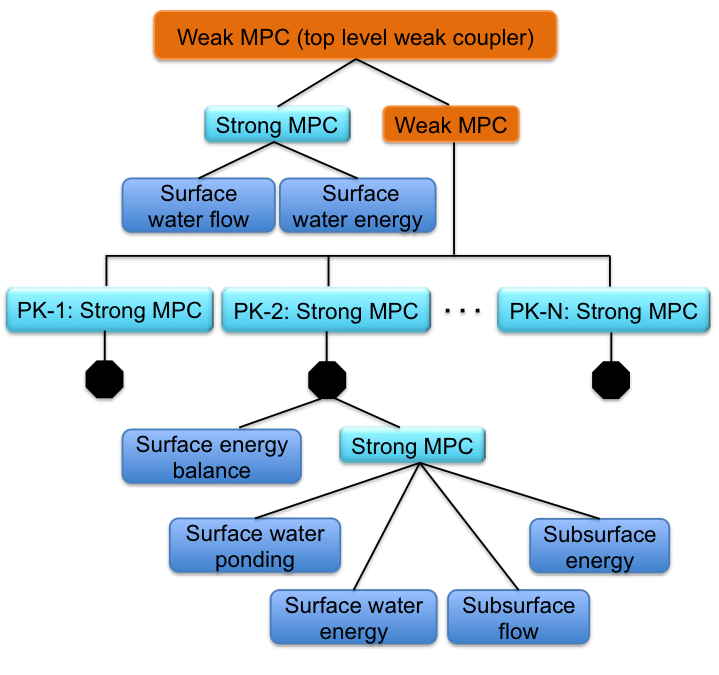
\includegraphics[height = 7.5cm, width=11cm]{figures/process-tree1.png}
\caption{A customized hierarchical structure of the process kernels. Blue blocks highlights independent process models; Light blue blocks strongly coupled independent process kernels; Orange blocks represent weak couplers.}
\label{pk-tree}
\end{figure}


\subsection{Weakly Coupled Scheme}
The weakly coupled scheme for analyzing our mixed-dimensional model involves two fundamental steps. Step 1 solves surface-star thermal hydrology system without  any external and exchanged sources. Step 2 solves subsurface system with surface ponding but no lateral surface flow. The first step mainly acts as a spatial distributor of the mass and energy, that is, distribute the pressures and temperature values across 2D overland system, and its solution serves as initial condition for Step 2. That is, the surface-star system updates the subsurface system (one-dimensional columns) before the subsurface system advances in time. After the update from Step 1, we implicitly solve subsurface system with surface ponding but no surface lateral flow, and use the output of that half-step to update surface-star pressure and temperature for the next iteration in the algorithm. As depicted in Fig.~\ref{coupling-schematic}, the top and bottom blue spots represent 2D surface-star system and 1D subsurface columns, respectively, and the cyan colors (in the middle) are intermediate steps for updating surface-star and surface/subsurface systems. For the sake of clarity, we will refer to the pressure and temperature fields of step 1 as surface-star pressure and temperature, while that of Step 2 will be called as subsurface and surface pressures and temperatures.


%\textbf{Refer to some published work related to mixed-dimensional modeling.}

\begin{figure}[!htpb]
\centering
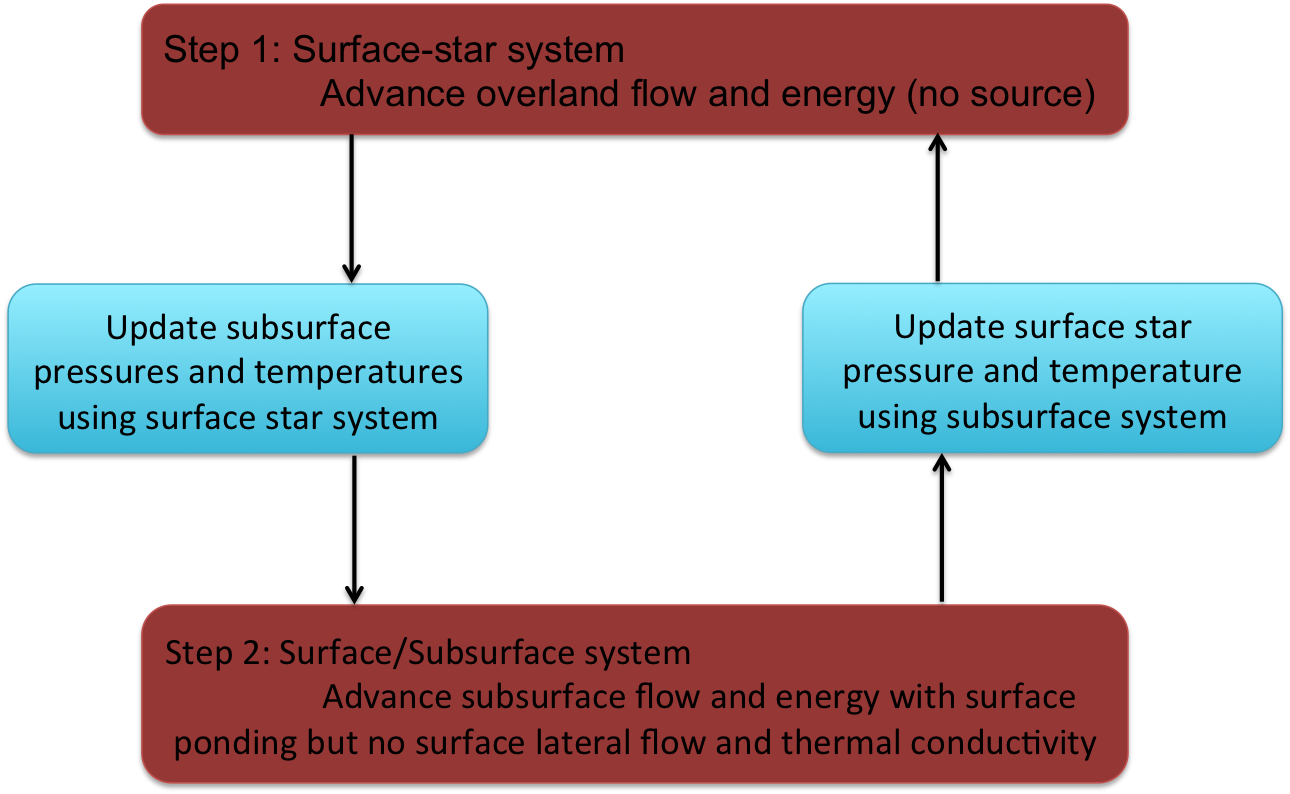
\includegraphics[height = 6.5cm, width=11cm]{figures/coupling-scheme.png}
\caption{Schematic of the loosely coupled scheme for our mixed-dimensional model. Brown represents advancement of PKs in time; Cyan shows intermediate steps for initialization of PKs within a single iteration.}
\label{coupling-schematic}
\end{figure}


\subsection{ATS Refactoring Strategy}
The ATS was significantly refactored to accommodate the above customized weak MPC. The refactoring allows PKs to be replicated across multiple subdomains (meshes), that is, each PK is state independent. This stateless structure permits each surface and subsurface subdomain to have its own domain name, say 
column$\_n$, surface$\_$column$\_n$, $n=1,2,3, \dots$, N. In fact, the refactoring strategy prefixes the variables (primary, secondary, and independent) with their corresponding subdomain names (e.g., column$\_n$-pressure, column$\_n$-temperature, $n=1,2,3, \dots$, N) -- that yields each PK in its most general form. These generic PKs now allow to construct any type of customize MPC for mixed-dimensional modeling technique.

Complexity of the multiphysics PK tree in our modeling strategy could not have been achieved without the Arcos framework. Though the complexity in the PK tree is evident but additional complications are intended as we include more processes (physical, chemical, biological and geological processes) and their mutual interactions. All these processes are equally important for an accurate and reliable long-term projections of permafrost regions. That said, the refactored ATS is more effective in addressing important challenges in the permafrost thawing in warming climate.


\section{Results and Discussions}\label{numerical-tests}

In this section, we present numerical results that highlights the accuracy and efficiency of our modeling technique. At the development stage, several numerical experiments were performed to verify the physical behavior of the refactored modules (PKs) of the ATS, code verification details are presented in~\ref{code-verification}. The spinup process (i.e., model's initialization) has been described in detail in~\cite{spainter2016integrated}. 


\subsection {Numerical Results -- A Comparative Study} 
To demonstrate the accuracy of our modeling technique, we compare numerical results of the mixed-dimensional model against a fully coupled three-dimensional simulations that act as a benchmark for our simulations. The domain under consideration has surface elevation varying between 4.14-4.62 m, enclosed by a horizontal plane 173 $\times$ 160 m$^2$, and 40 m deep; see Fig.~\ref{surf-location}. This domain is a part of the low-gradient polygonal tundra in Barrow, Alaska and consist of 75 general polyhedra. As highlighted in Fig.~\ref{surf-location}, we select five spots (based on different elevations) to perform a location-based comparison of the numerical results of the two schemes. 
\begin{figure}[!htpb]
\centering
%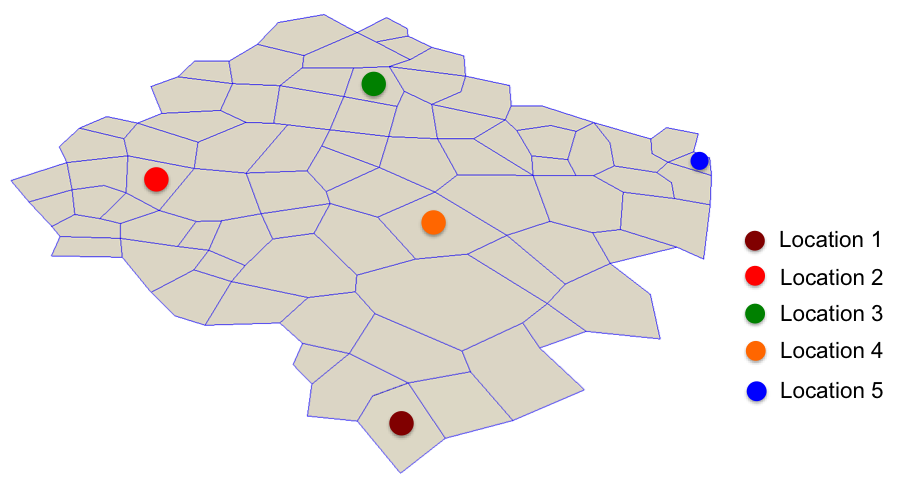
\includegraphics[height = 5.5cm, width=9cm]{figures/surface-locations.png}
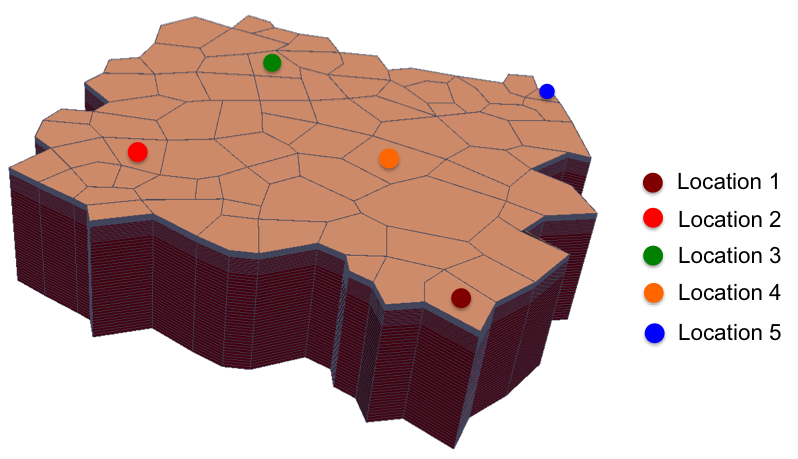
\includegraphics[height = 6.5cm, width=11cm]{figures/lobster75-3d.png}
\caption{An illustration of the five spatial locations on 75 polygons cluster for location-based comparison of the two schemes. Location 1: Outlet. Location 2: High elevated spot. Location 3-4: Intermediate elevation spots. Location 5: Lowest elevation spot.}
\label{surf-location}
\end{figure}
We demonstrate three set of studies based on the variations introduced in the surface elevation. We use the following equation to exaggerate the surface topography,
\begin{equation}\label{formula-exagg}
\bar{Z} =  \alpha (Z - \mu) + \mu.
\end{equation}
Here $\bar{Z}$ is the exaggerated elevation, $Z$ is the original elevation with mean $\mu$, and $\alpha$ is the exaggeration parameter. Equation~(\ref{formula-exagg})  preserves the mean while the standard deviation depends on the value of $\alpha$ and is given by $0.14 \alpha$. The coefficient in front of $\alpha$ is the standard deviation of the original elevation $Z$ -- in our case $Z$ correspond to the domain shown in Fig.~\ref{surf-location}. Our three set of studies correspond to $\alpha=1,3,$ and $5$.
These studies aim to determine (in an approximate sense) the failure of the mixed-dimensional model. In other words, since our modeling strategy is mainly based on a loosely coupled scheme thereby it should eventually results in breakdown due to significant heterogeneity in the surface elevations. We expect the model to give promising results for simulating low-gradient polygonal tundra, and believe that the values of $\alpha$ we choose provide reasonably enough variations for a domain of 100s of meter. For the sake of clarity, hereafter, we refer to the cases of $\alpha = 1, 3$ and $5$ as Study-I, II and III, respectively. \\
Our numerical experiments confirm a high agreement between the results of the mixed-dimensional model and the 3D model at all selected location for all three studies. We present the results of study I in more detail, and it serves as a representative of the other two studies. Also, most of the presented plots correspond to the early summer. Fig.~\ref{ss-sat-comp} and~\ref{ss-temp-comp} compares the subsurface water saturations and temperatures at locations 1 and 5, respectively. The accuracy of our results is evident. The surface ponded depths of the two models are depicted in Fig.~\ref{surf-pd-comp}.  We compare the surface temperatures obtained with the two-schemes in Fig.~\ref{surf-temp-comp} at locations 1 and 5. Fig.~\ref{surf-temp-comp} also displays the difference in the surface temperatures at the two locations highlighting spatial variability in the temperatures. As expect, our results fit the 3D model's results very well. We see the same level of agreement at the other locations as well, but we are not showing them here.
The root mean square difference in the subsurface water saturations of the two models of study-I, II, and III are shown in Fig.~\ref{error-plots}. Not surprisingly, as the value of $\alpha$ increases the error grows to some extent, but we still see the results of the mixed-dimensional model converge to the corresponding benchmark solution. The consistency of our numerical results with the fully coupled 3D simulations validate the accuracy of our scheme. 


% Fig 7. change title -- subsurface WATER saturation

% add Study I, II and III to the titles


 \begin{figure}[!htpb]
\centering
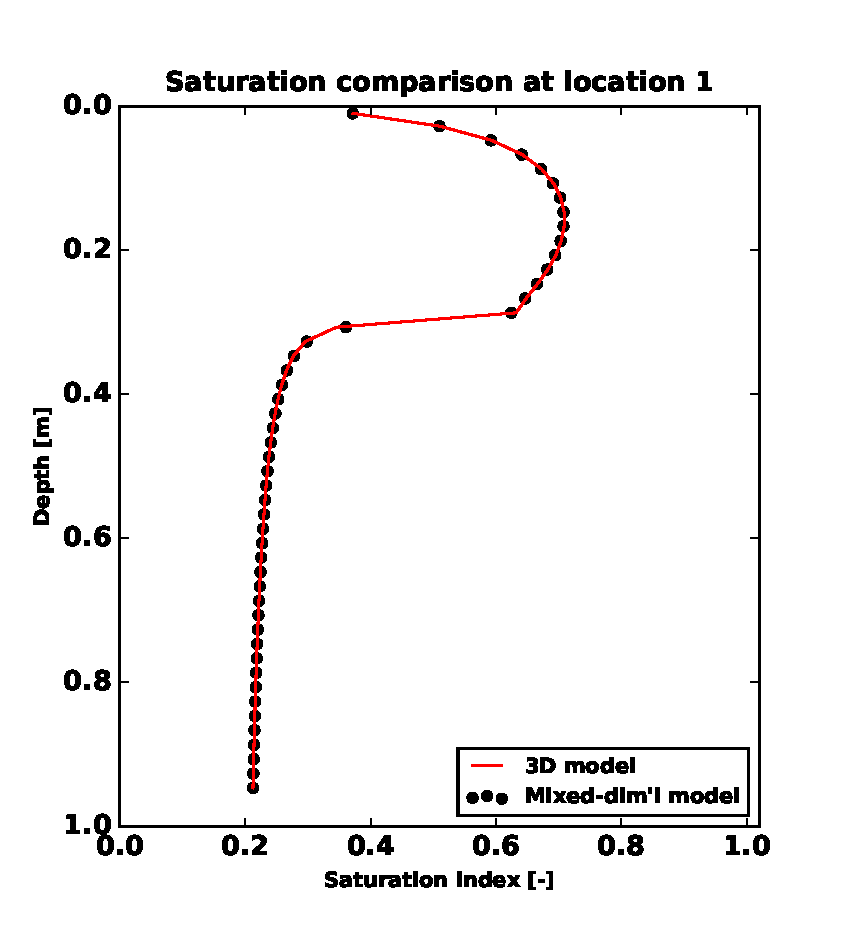
\includegraphics[height = 7.5cm, width=6cm]{figures/comparison/regular/ss-sat/comp-sat-loc1-cycle0020.eps}
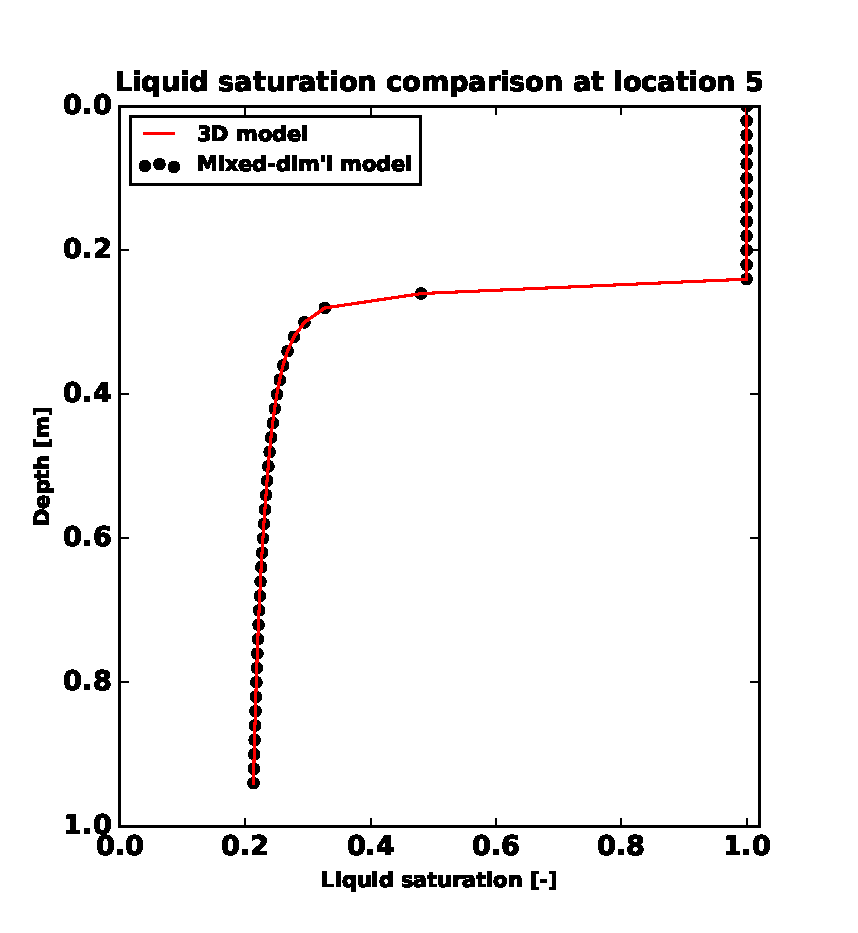
\includegraphics[height = 7.5cm, width=6cm]{figures/comparison/regular/ss-sat/comp-sat-loc5-cycle0020.eps}
\caption{Comparison of the subsurface water saturation at locations 1 and 5 during the summer.}
\label{ss-sat-comp}
\end{figure}


\begin{figure}[!htpb]
\centering
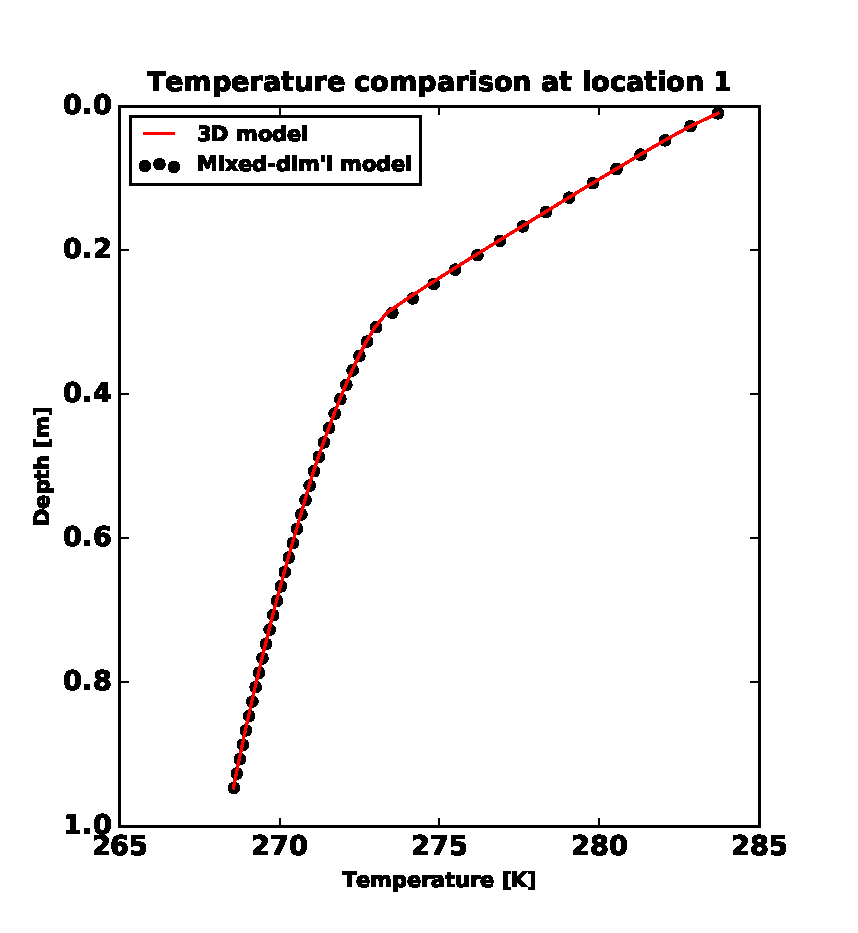
\includegraphics[height = 7.5cm, width=6cm]{figures/comparison/regular/ss-temp/comp-temp-loc1-cycle0020.eps}
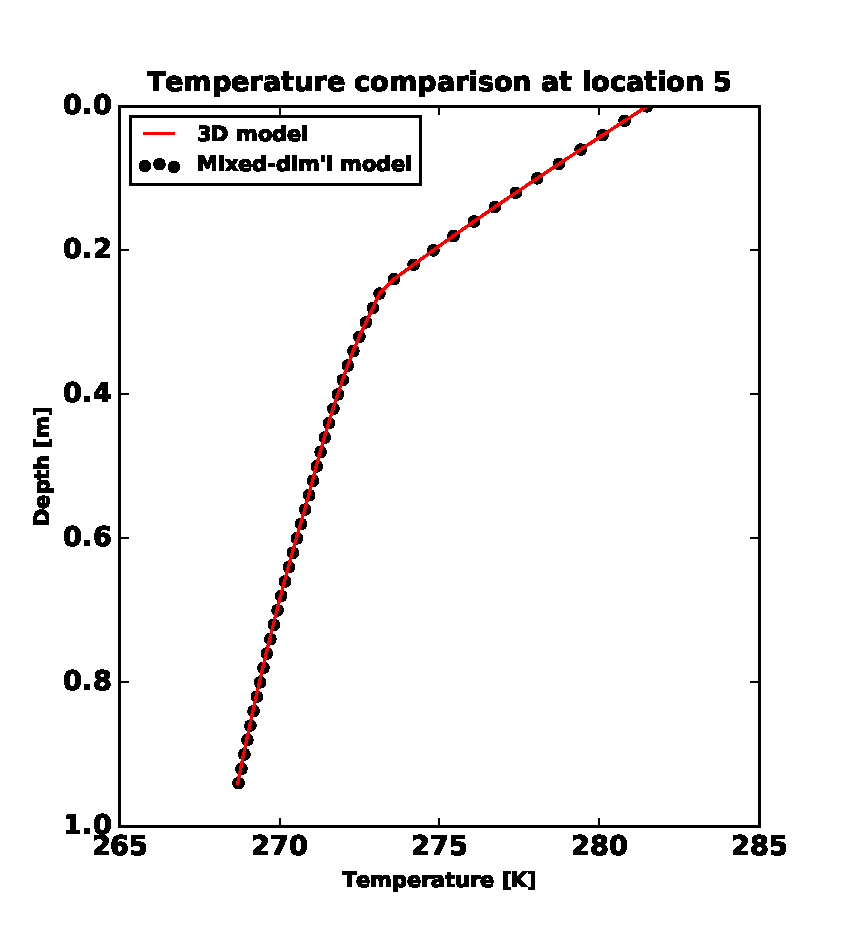
\includegraphics[height = 7.5cm, width=6cm]{figures/comparison/regular/ss-temp/comp-temp-loc5-cycle0020.eps}
\caption{Comparison of subsurface temperatures at locations 1 and 5 during the summer.}
\label{ss-temp-comp}
\end{figure}

\begin{figure}[!htpb]
\centering
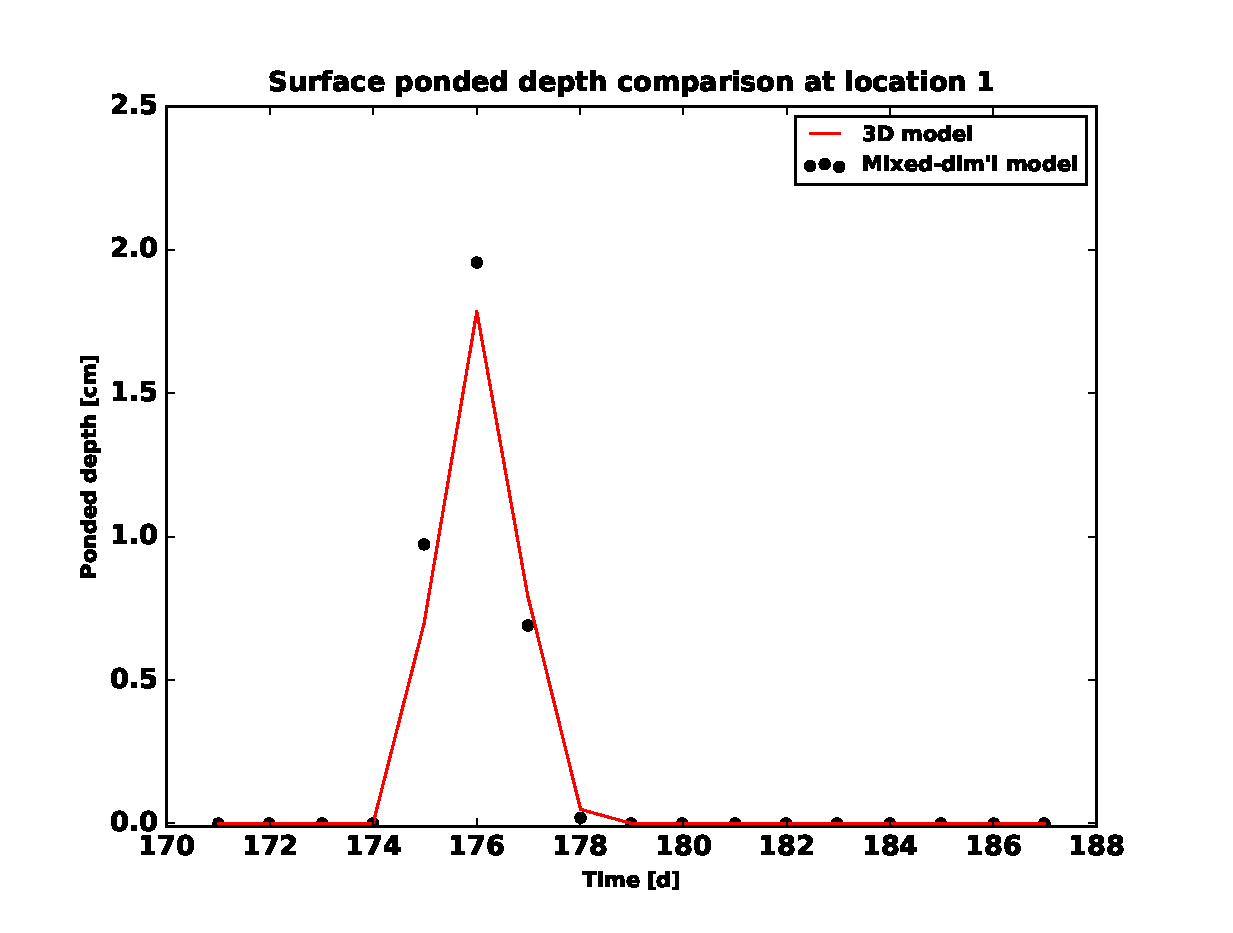
\includegraphics[height = 7.5cm, width=6.cm]{figures/comparison/regular/ponded-depth/comp-pd-location1.eps}
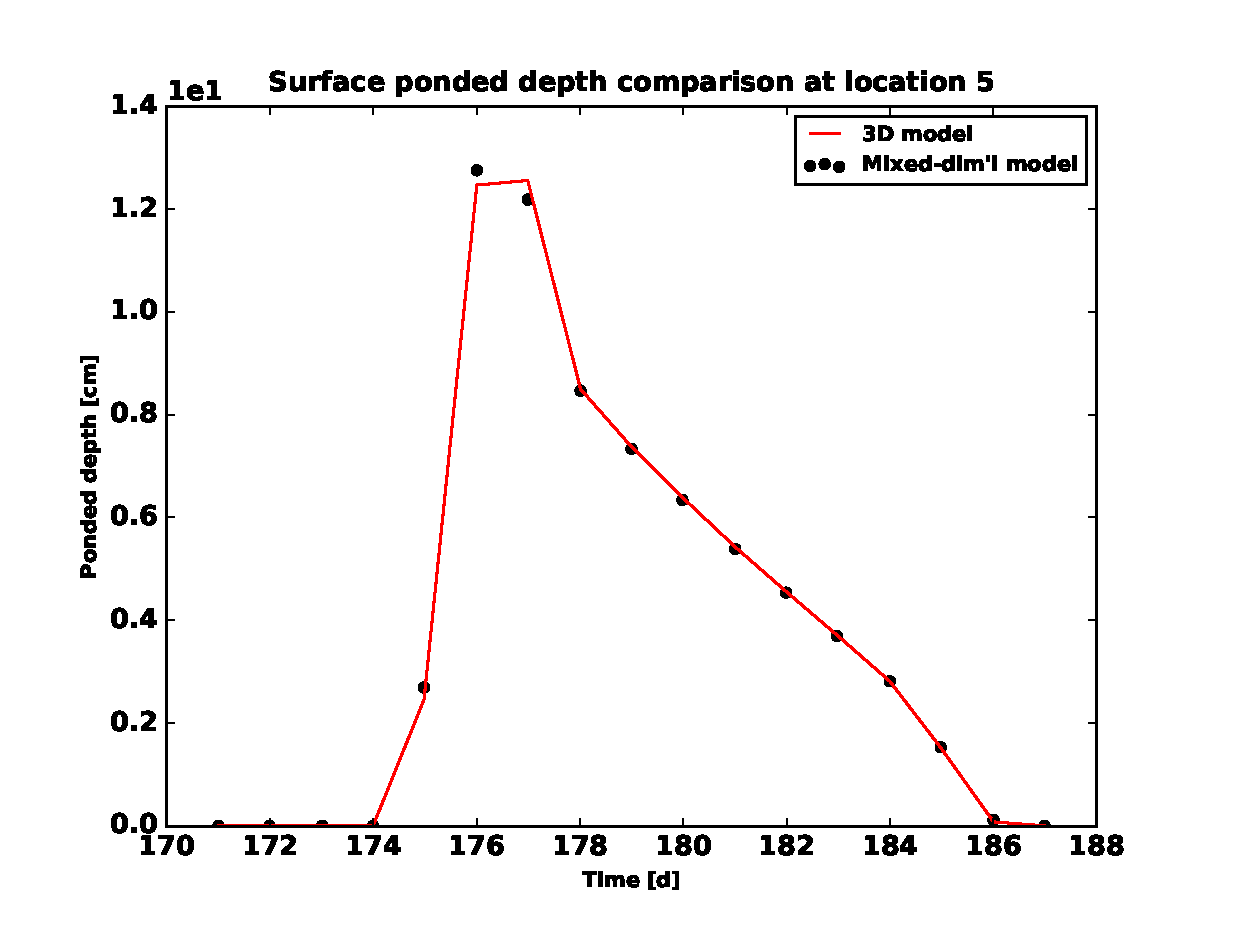
\includegraphics[height = 7.5cm, width=6.cm]{figures/comparison/regular/ponded-depth/comp-pd-location5.eps}
\caption{An illustration of the surface ponded depths of the two schemes at locations 1 and 5 when the snow melt starts.}
\label{surf-pd-comp}
\end{figure}

\begin{figure}[!htpb]
\centering
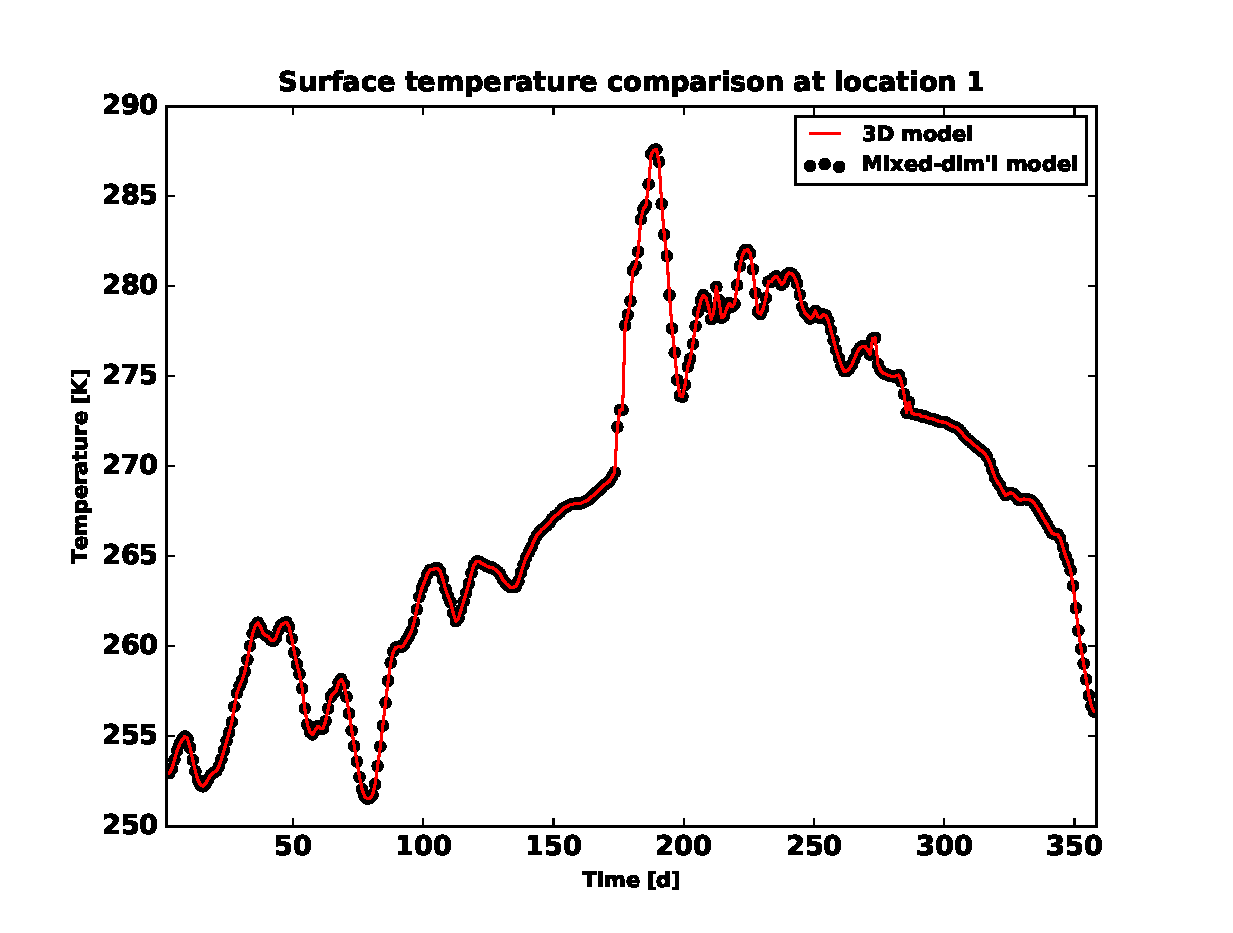
\includegraphics[height = 5.9cm, width=11.cm]{figures/comparison/regular/surf-temp/comp-temp-location1.eps} \\
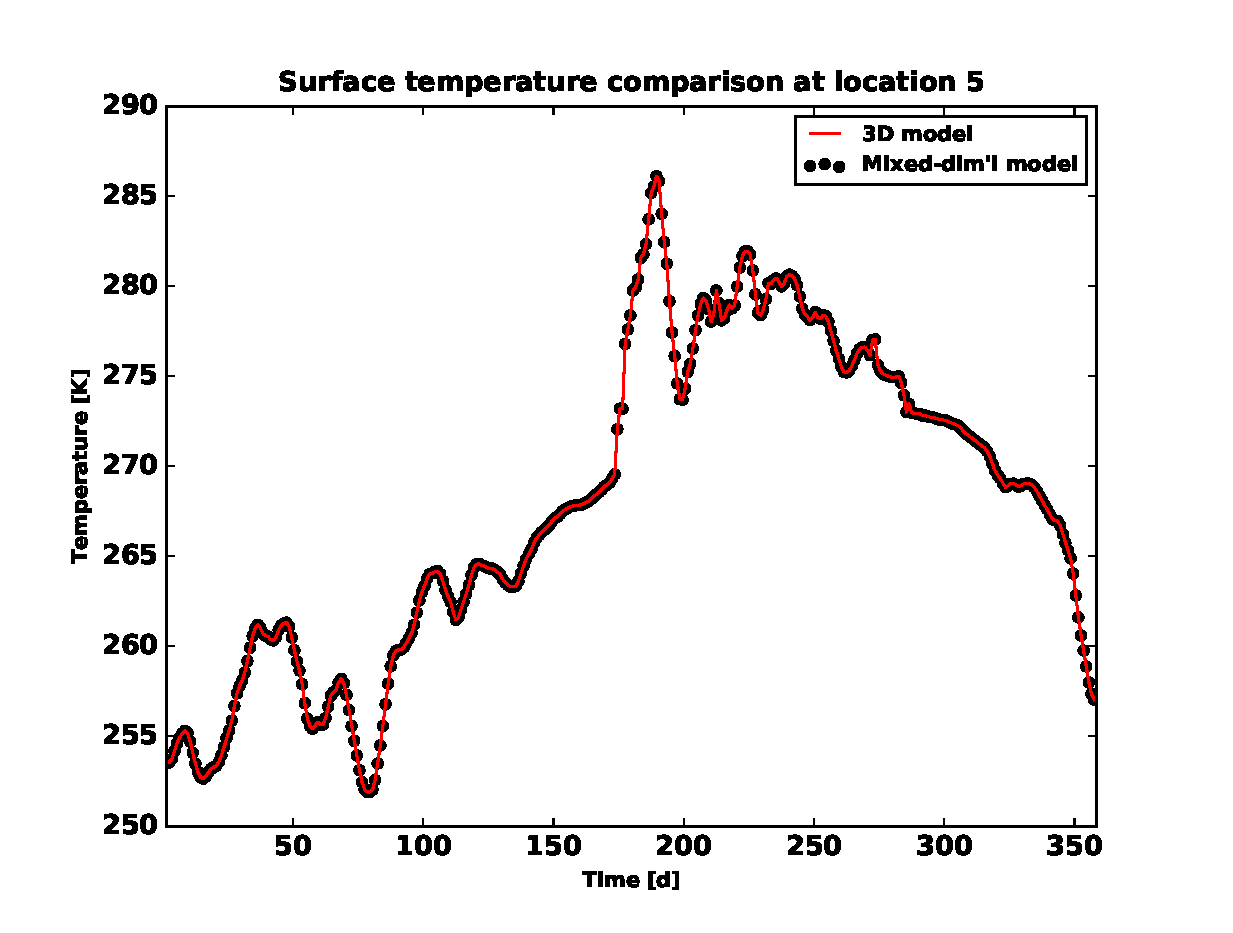
\includegraphics[height = 5.9cm, width=11.cm]{figures/comparison/regular/surf-temp/comp-temp-location5.eps}
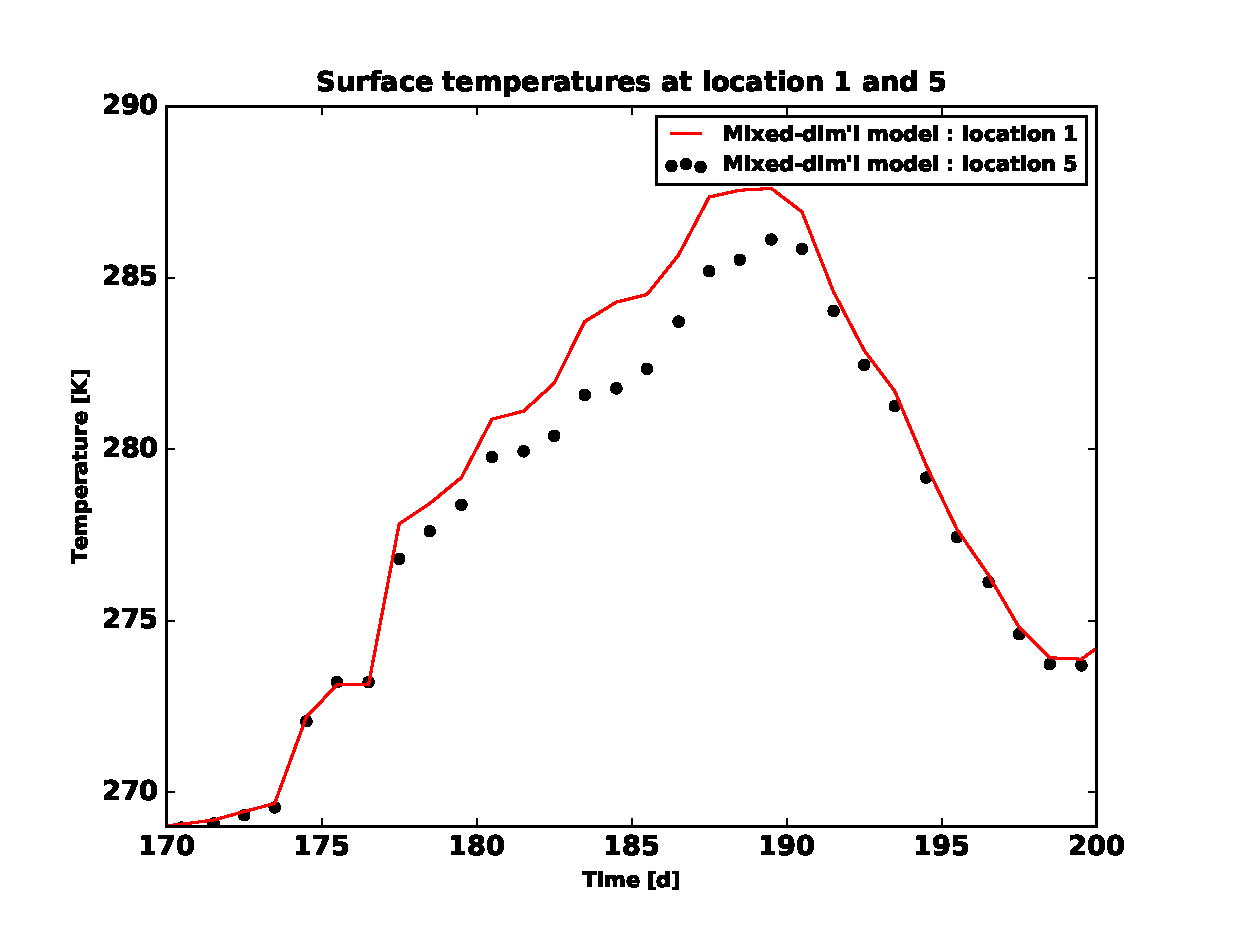
\includegraphics[height = 5.9cm, width=11.cm]{figures/comparison/regular/surf-temp/comp-temp-location1-5.eps}
\caption{An illustration of the surface temperatures of the two schemes at locations 1 and 5 for the entire year. The bottom plot highlights the difference between the temperatures at location 1 and 5, though they appear quite similar in the top two plots.}
\label{surf-temp-comp}
\end{figure}


\begin{figure}[!htpb]
\centering
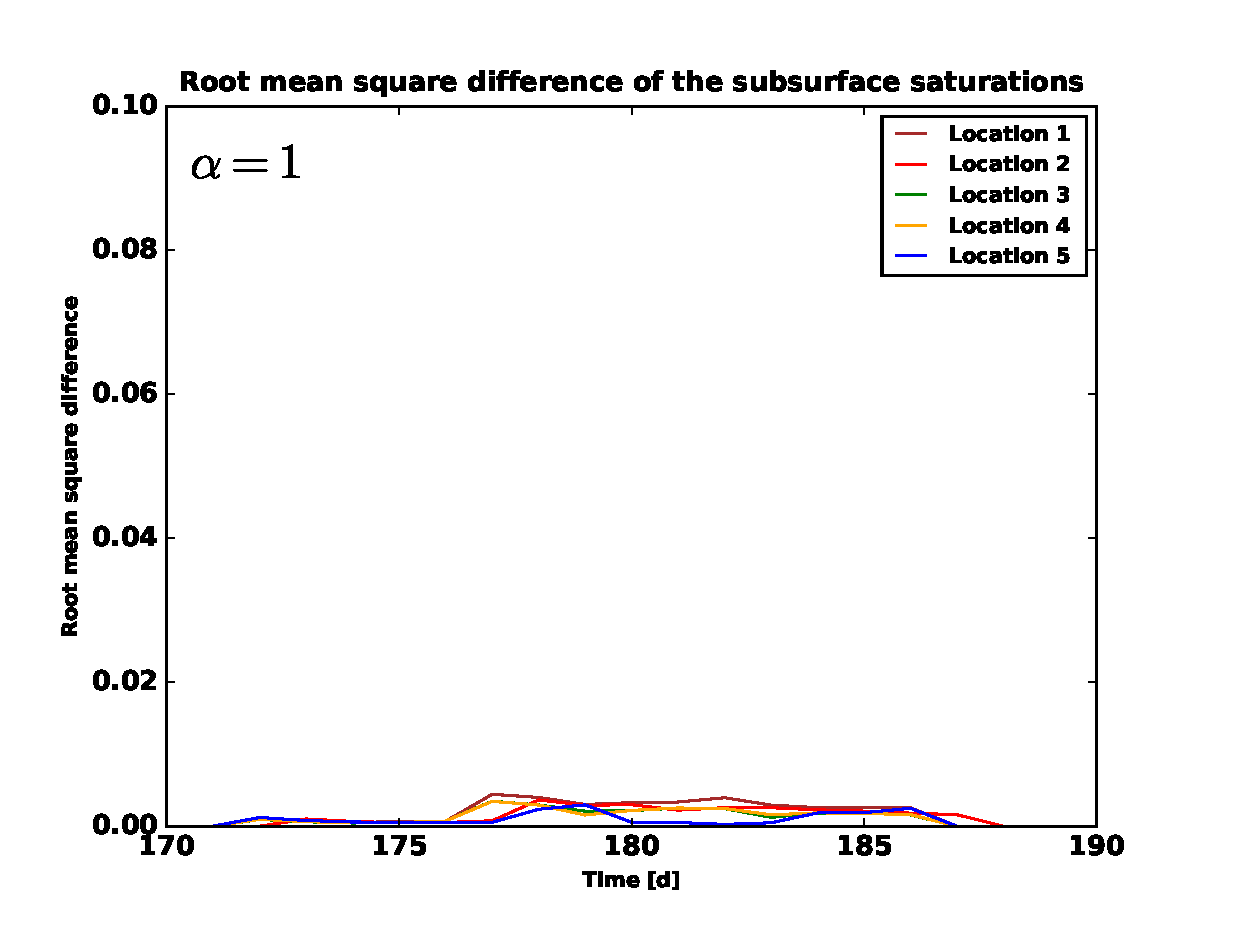
\includegraphics[height = 6.cm, width=10.cm]{figures/comparison/regular/error.eps}
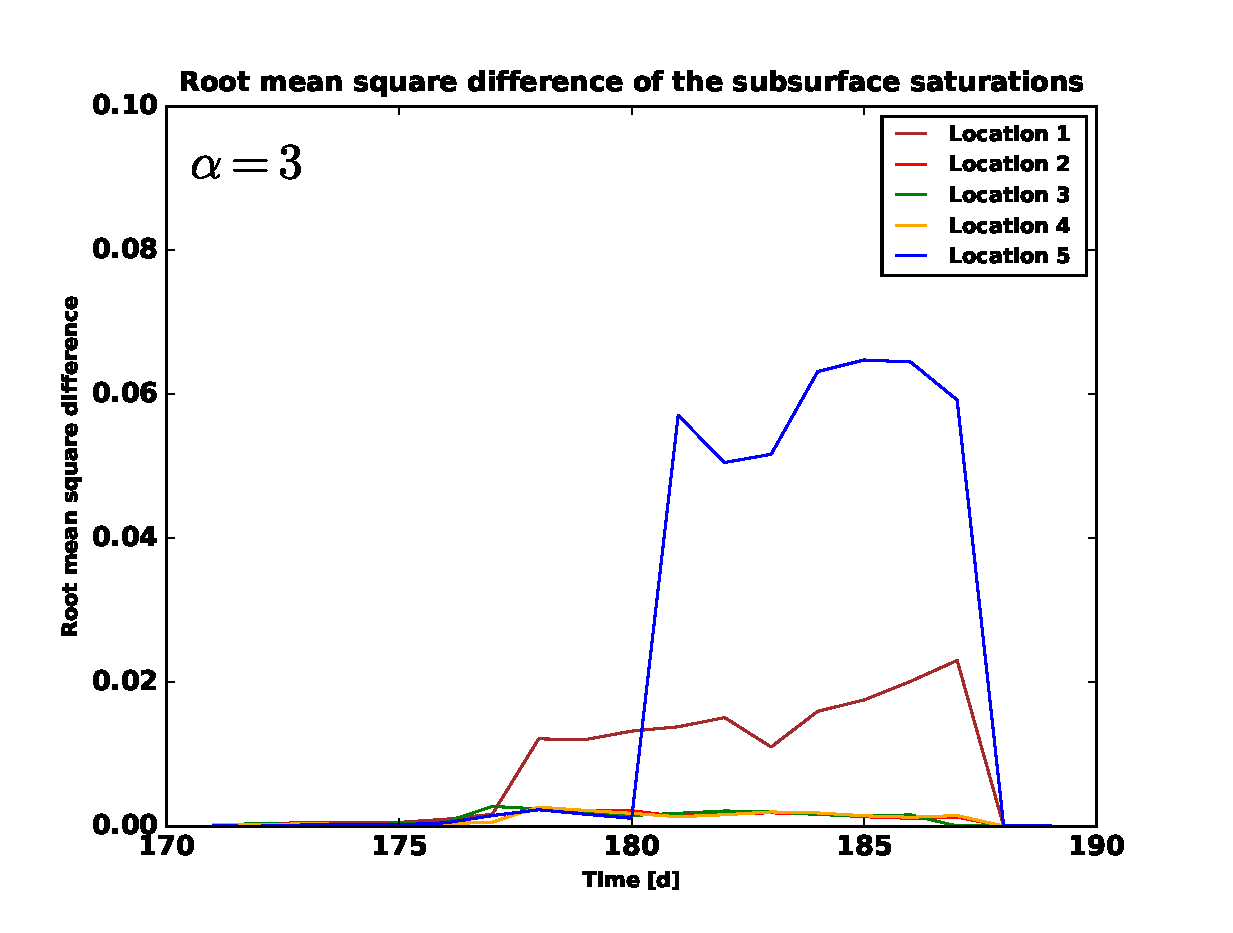
\includegraphics[height = 6.cm, width=10.cm]{figures/comparison/dist/Elev-grad1.5m/error.eps}
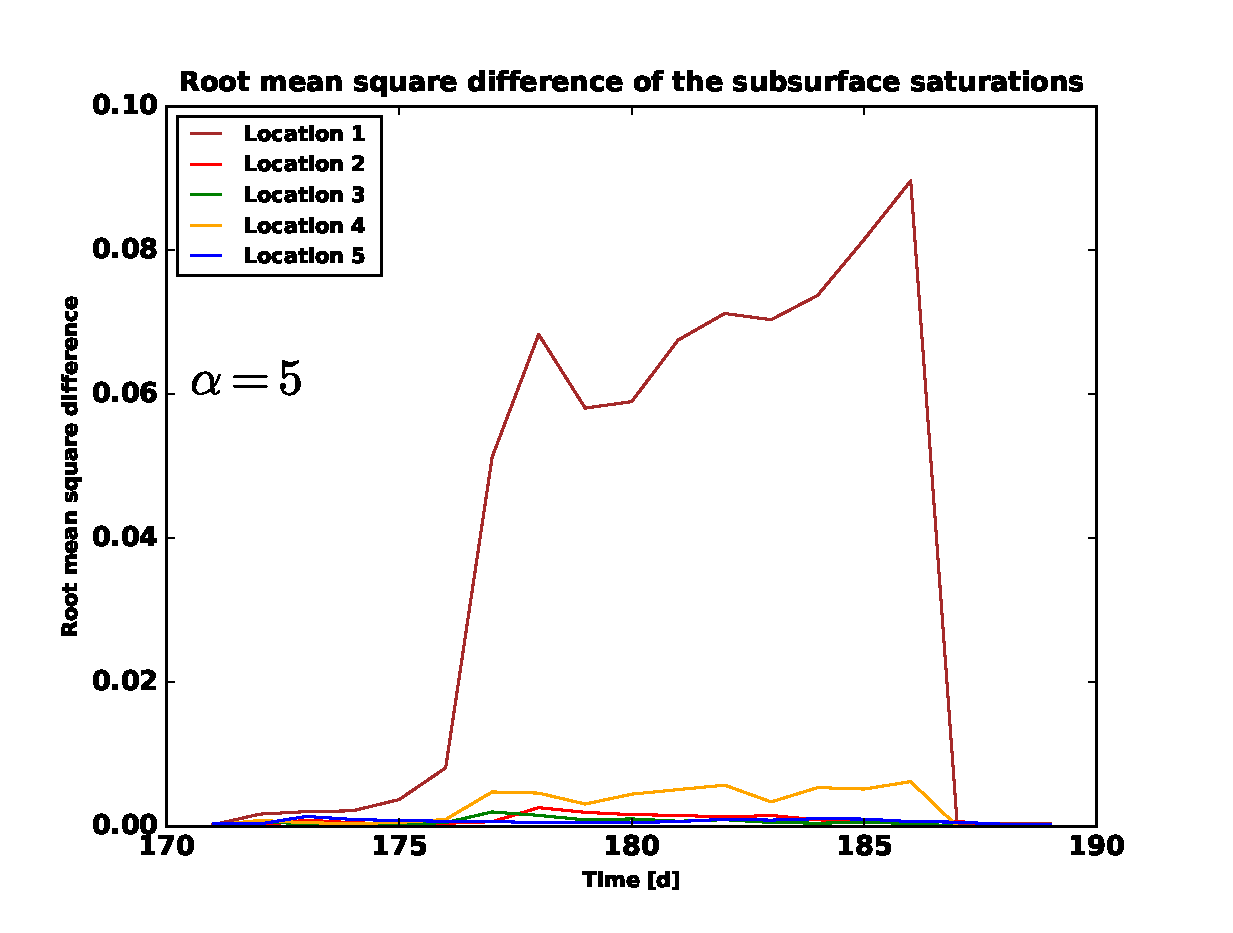
\includegraphics[height = 6.cm, width=10.cm]{figures/comparison/dist/Elev-grad2.5m/error.eps}
\caption{The root mean square difference of the subsurface water saturations at the selected locations of the three studies.}
\label{error-plots}
\end{figure}


%\todo{should we provide a Table describing Parameters used in the simulations}

\subsection{Speedup Study}
We discuss speedup study for two spatial domains -- one with 75 polygons as depicted in Fig.~\ref{surf-location} and the other one (not shown here) consists of 468 general polyhedra that is about 6-7 times larger than the first one. We highlight two aspects of the efficiency of our modeling approach: (i) how the simulation time decreases in comparison with three-dimensional simulations; (ii) how efficiently it scales? Figs.~\ref{3d-lcs-speed} compare the computational time of the two modeling approaches for the domain consisting 75 polyhedra.
It can be seen that for a fixed number of processors, the computational time decreases by a factor of about 4 with our modeling technique. This is a huge computational advantage without sacrificing the numerical accuracy. We show the speedup study for the aforementioned domains in Fig.~\ref{lcs-speed}. We see that the framework scales up better for larger domain. A considerable improvement pertaining to computational time and resources is expected with increasing size of the spatial domain. Ideally, one would want to employ the same number of processor as that of the subsurface columns to achieve the maximum efficiency, however, with increasing number of processors, the cost of interprocessor communication in the overhead 2D domain (i.e., the surface-star system) also increases and hence supersedes the performance. Overall, our novel modeling approach significantly reduces computational time without degrading numerical accuracy.
 
\begin{figure}[!htpb]
\centering
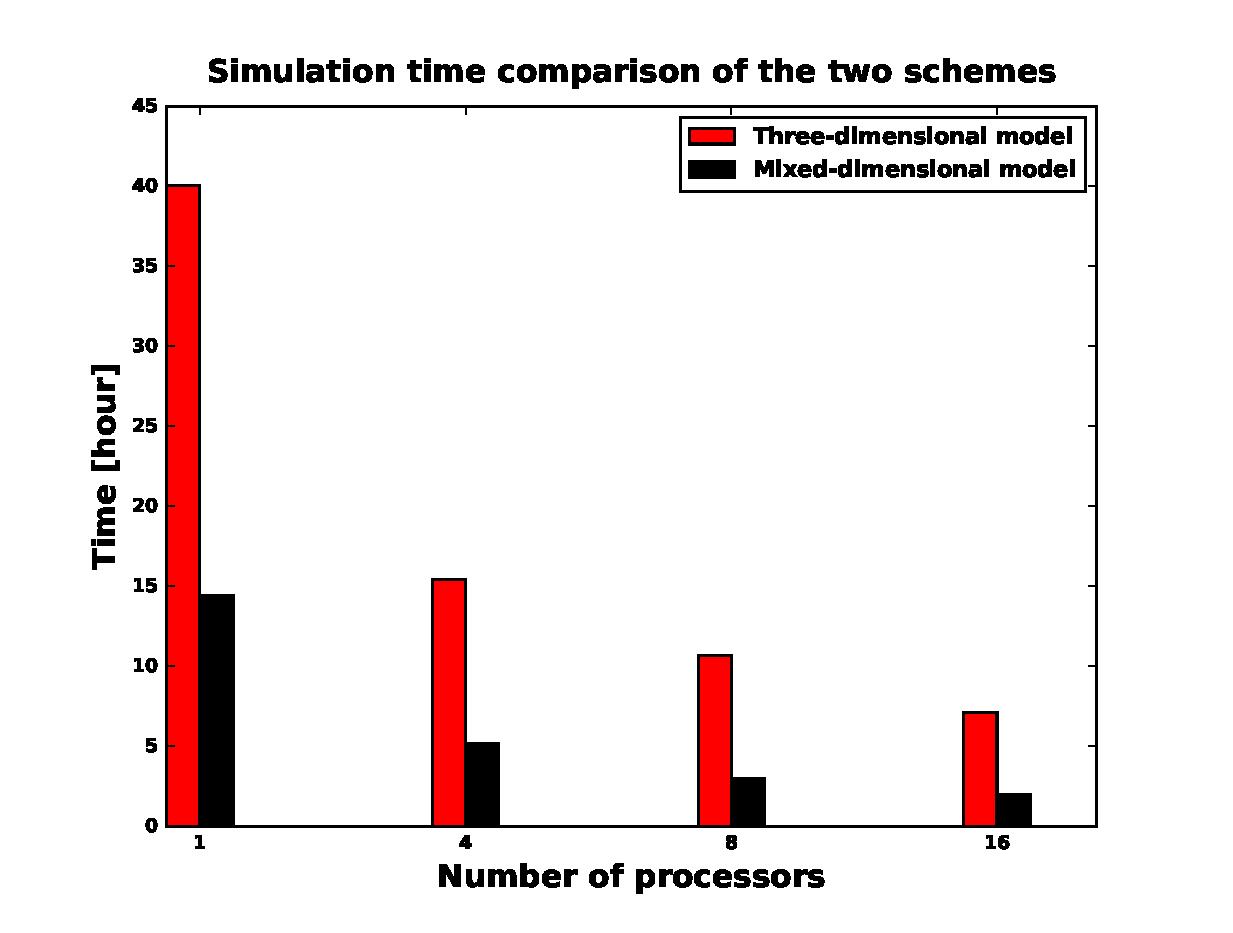
\includegraphics[height = 6.5cm, width=10cm]{figures/compare3d-lcs-speed.eps}
\caption{A comparison of the computational time taken by the mixed-dimensional and 3D models.}
\label{3d-lcs-speed}
\end{figure}


\begin{figure}[!htpb]
\centering
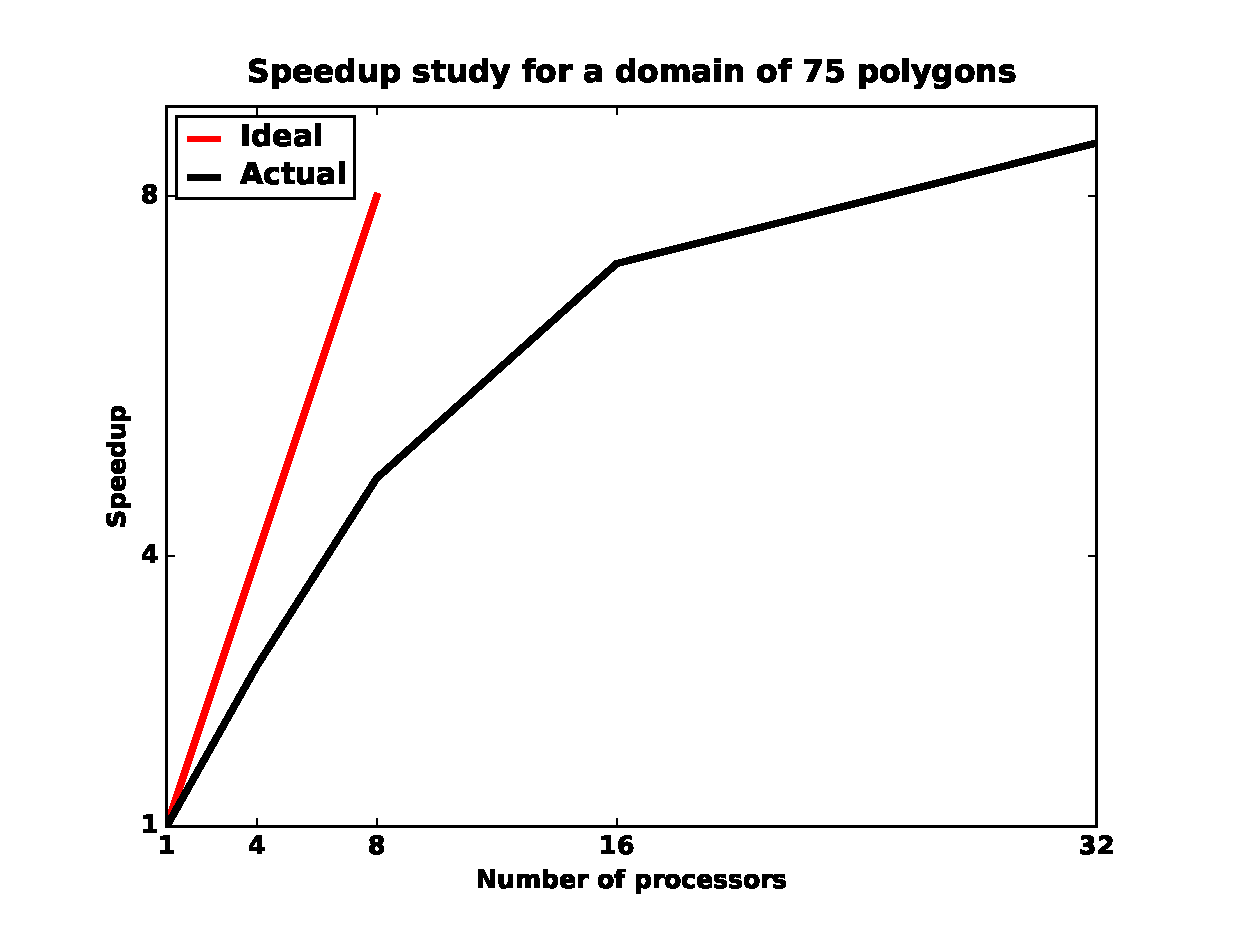
\includegraphics[height = 6.5cm, width=10cm]{figures/speedup-lcs-lobster.eps}
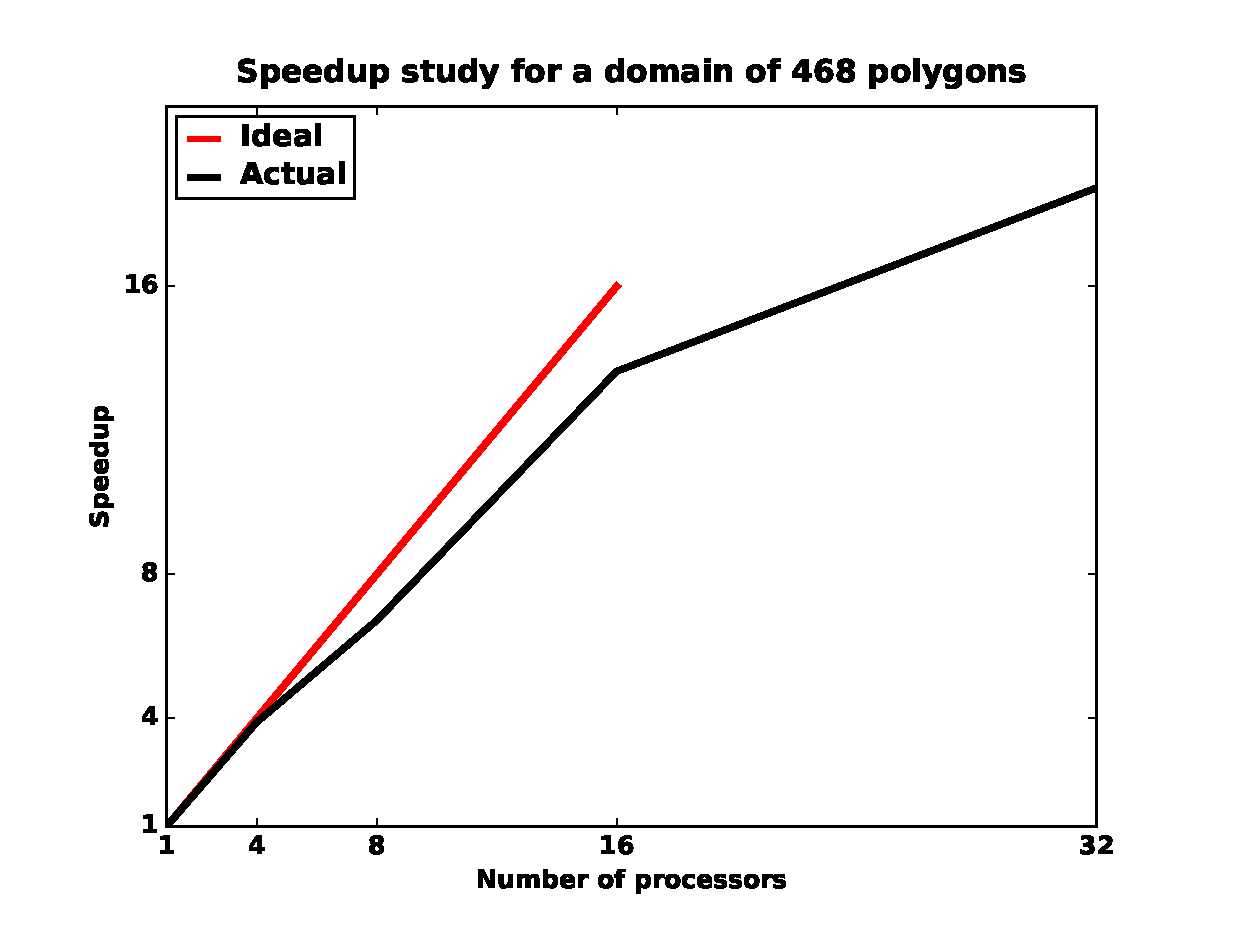
\includegraphics[height = 6.5cm, width=10cm]{figures/speedup-lcs-barrow.eps}
\caption{An illustration of the speedup study of a simulation with 75-polygon cluster (top) and 468 polygons barrow watershed (bottom).}
\label{lcs-speed}
\end{figure}

\subsection{Subcycling Process Kernels}
Subcycling is a multi time stepping approach in simulations. The idea is to assign a suitable local time-step to each subdomain rather than one single global time-step. The subcycling is a very convenient approach for simulating permafrost type regions because during the time of snowmelt and snow accumulation, the time-step of the numerical methods is relatively smaller, and a reasonable amount of computational time is spent during these periods. Further, in permafrost simulations, due to the spatial variations in the thermal and hydrological conditions the phase change is mainly local, but its affects are global pertaining to the time-step. \\
Our mixed-dimensional modeling approach efficiently allows subcycling PKs because we discretize subsurface as independent columns/subdomains. Thereby the subdomains can advance in time with their preferred time-steps until they hit the synchronized time. We see a 15-20\% decrease in the computational time as compared to no subcycling simulations. We intend to explore this topic and report a detailed study in near future as we believe the subcycling approach should significantly reduce computational time.

\section{Conclusions and Future Work}\label{conclusion}
\subsection{Closing Remarks}
We present a novel mixed-dimensional modeling approach that is mainly based on discretizing subsurface as independent columns and then indirectly coupled to a two-dimensional surface system. This approach has motivated by fine-scale simulations of permafrost regions that explored spatial variations in the thermal conditions among centers, rims, and troughs of ice-wedge polygons during the summer, and mainly equilibrated by lateral heat transport.
%Though this modeling approach has a broader scope but we mainly focus on simulating the thermal hydrology of degrading permafrost (polygonal tundra) near Barrow, Alaska.

Simulating a fully integrated surface and subsurface thermal hydrology in permafrost-affected regions is both important and challenging. The importance lies in the fact that permafrost stores massive amount of organic carbon and the degree of warming in these regions is a few times greater than the global mean. That said, these regions may become a major contributor of carbon release to the atmosphere in warming climate. The strong coupling among thermal and hydrologic processes on the surface and in the subsurface, permafrost degradation, numerical issues, and large-scale projections make these simulations significantly challenging. \\
This is a very first attempt to couple state-of-the-art representation of freezing soil physics with overland flow and surface energy balance at scales of 10s of meters.  Our novel mixed-dimensional modeling approach is implemented in state-of-the-art Arctic Terrestrial Simulator (ATS). The ATS is an open-source simulator, leverages Amanzi (a flow and transport simulator) and uses Arcos framework. The Arcos framework manages the process kernels (a mathematical model) in a hierarchical structure, and couples many independent processes through a Multiprocess Coordinator (MPC). It allows the flexibility of extending existing modeling capabilities, and provides highly suitable environment for managing complexity in the process-rich simulations.

The coupling algorithm for analyzing our mixed-dimensional model has two fundamental steps. The first step solves a two-dimensional surface thermal hydrology system, that spatially distributes mass and energy, and initializes subsurface system at each time-step. The second step solves an integrated subsurface and surface ponding system, and at the end it updates surface system for next time-step.

We compare our numerical results with a fully coupled surface and subsurface scheme to demonstrate the efficiency and accuracy of our modeling approach. The fully coupled scheme acts as a benchmark for our scheme. Numerical results show our scheme is computationally more efficient and as accurate as a fully coupled scheme. 

Our modeling approach has many advantages over existing hydrological simulators. Many available simulators are designed to work with a single spatial domain, don't support subdomains modeling techniques, large-scale deformations, flexible future extensions. Our modeling technique does not pose such limitations on simulating process-rich permafrost dynamics. We can effectively incorporate many processes (physical, chemical, biological and geological processes) and let them interact through MPCs. The scheme is computationally more efficient, accurate and scalable. In addition, it can efficiently track thaw-induced subsidence, allows subcycling individual subdomains, and avoids any mesh tangling and poor mesh quality that can result from representing dynamic topography in a three-dimensional simulation.
 

 
\subsection{Future Directions}
This is a first attempt to provide process-rich simulations capability of the permafrost regions at watershed-scale. However, the work is not yet complete, we intend to  extend this capability to address more challenging problems in the near future. A very first task would be to incorporate a subgrid model for dynamic microtopography. Thawing of permafrost can cause ice-wedge polygons to deform, mold and change the landscape (low-centered polygons can transform to high-centered polygons)~\cite{jorgenson2006abrupt,liljedahl2012ice}. Further, it can bring substantial changes in hydrology and soil moisture, can alter the drainage network, and transform a dry region to a wetland ecosystem~\cite{hinzman2005evidence,rowland2010arctic}. Our modeling strategy is designed in a way that can easily allow to track thaw-induced subsidence in simulating permafrost dynamics, because we are mainly working with one-dimensional columns (i.e., the discretization is based on independent 1D columns).




%\section{Bibliography styles}

\appendix
\section{Numerical Experiments -- Code Verification}\label{code-verification}
We have performed a series of tests at the development stage for code verification, and compared our results against numerical solution of three-dimensional model. The 3D results serve as a benchmark for our scheme. In 3D models the surface and subsurface systems are strongly coupled and solved implicitly. Since our model required major refactoring of the ATS, so individual pieces of the code were deeply tested before integration -- they are listed below:
\begin{itemize}
\item{ Problem Test 1 (Subsurface Flow): 
We consider multiple subsurface columns with flat top surface -- each column is an independent domain. Put water table below the surface, infiltrates and fills the subsurface columns.
}
\item{ Problem Test 2 (Surface and Subsurface Flow only): 
This is an extension of the Test 1. We Put water table below the surface. Water infiltrates and fill subsurface columns prior to surface ponding. 
}

\item{ Problem Test 3 (Subsurface Thermal Hydrology): 
We add energy equation to Test 1. Initially, establish water table close to the surface, and start freezing from below. The frozen subsurface columns are thawed from the top.}

\item{ Problem Test 4 (Surface and Subsurface Thermal Hydrology):
In this test, we incorporate surface thermal hydrology into Test 3. A warm rain precipitation thaws the subsurface columns, saturate them and afterwards water ponds on the surface.}

\item{ Problem Test 5 (Surface Energy Balance, Surface and Subsurface Thermal Hydrology):
A fully integrated surface and subsurface processes test. We introduce an energy balance equation to Test 4. An initially established ice table below the surface has been thawed by warm rain, incoming-short radiation and air temperature.}

\end{itemize}
Due to symmetry in the domains of above numerical tests, that is, the subsurface columns are copies of each other and surface is flat, we get identical results and compare very well with its corresponding three-dimensional simulation results. Passing all the above tests conclude refactoring of the ATS a success. In the preceding discussion, we consider general polyhedra due to the polygonal structure of the Arctic landscape.


\section*{References}

\bibliography{reference}

\end{document}



\subsection{Spinup Process}
Spinup \todo{ we describe this in our ATS overview paper, so should eliminate and cite} refers to a sequential process that initializes model's domain to make it consistent with current climate before driving it with meteorological forcing data for future projections. We take the following steps to spinup the model:
\begin{itemize}
\item{ Step 1. Establish a water table close to the surface in a one-dimensional subsurface column by running a steady-state Richards flow.}
\item{Step 2. Freeze the water table from below (set the bottom boundary condition below freezing) -- leading to an ice table in the subsurface column. Since water expands on freezing, therefore, from numerical point of view, the idea is to place the water table at a location such that the ice table remains below the surface.}
\item{Step 3. Initialize the entire subsurface domain using one-dimensional column data, that is, map the 1D column data to the whole domain to establish an ice table.
}
\item{Step 4. Drive the model for 10 years -- a cyclic simulation with one year averaged meteorological data. The one year averaged data is obtained by aggregating the 10 years observed meteorological data, that is, the mean value of a forcing factor (say, air temperature, humidity etc.) for a specific day per 10 years. This completes a typical spinup process in ATS, that is, initialization of the model is done. Lastly, the model was forced by 10 years data due to the availability of the observed data from 1999 to 2009 at Barrow, Alaska -- the site of our interest in this work.}
 \end{itemize}
 
 
 %\begin{description}
%\item {Study-I:} Setting $\alpha  = 1$ gives the original (no exaggeration) topography. The elevation has mean 4.42 and standard deviation 0.13.

%\item{Study-II:} Topography has slightly exaggerated. The value of $\alpha$ is set to 3 that yields the topography with mean 4.42 and standard deviation 0.40.
%\item {Study-III:} Using $\alpha=5$ brings more variations in the surface topography. The exaggerated topography has mean 4.42 and standard deviation 0.67.  
%\end{description}
